\documentclass[12pt,twoside,a4paper]{article}
\usepackage{listings}
\usepackage{tcolorbox}
\usepackage{placeins}
\usepackage{hyperref}
\usepackage{float}
\newcommand{\lstfont}[1]{\color{#1}\scriptsize\ttfamily}

\lstset{
    language=[ANSI]C++,
    showstringspaces=false,
    backgroundcolor=\color{black!90},
    basicstyle=\lstfont{white},
    identifierstyle=\lstfont{white},
    keywordstyle=\lstfont{magenta!40},
    numberstyle=\lstfont{white},
    stringstyle=\lstfont{cyan},
    commentstyle=\lstfont{yellow!30},
    emph={
        cudaMalloc, cudaFree,
        __global__, __shared__, __device__, __host__,
        __syncthreads,
    },
    emphstyle={\lstfont{green!60!white}},
    breaklines=true
}


\title{GPU Computing\\
Exercise 5}
\author{
  Luis Wenzel\\
  Miro Joensuu\\
  Daniel Bayer\\
  Noah Schneider
}
\date{}

\begin{document}

\maketitle

\section{Presenting}
Willing to present:\\
6.1 \\
6.2 Yes\\
6.3 \\
6.4 \\
6.5 \\
6.6 \\

\newpage
\section{Reading}
The article introduces the roofline model, describing the maximum achievable performance, limited by memory bandwidth and computational capabilities, depending on the operational intensity of a given problem. The roofline consist of two main components: the memory bandwidth ceiling and the computational ceiling, although for both metrics multiple lines may be drawn into a diagram to represent different performance optimizations like software prefetching or the use of SIMD instructions. Fallacies of the model, e.g. ignoring features like caching, are discussed as well.\\
The article describes the roofline model as a performance guideline for processors of varying number of cores and complexity, showing how the operational intensity defines whether a problem is memory-bound or compute-bound. This then gives a direction which optimizations will have an actual impact on the performance. This allows for a discussion on performance behavior from not just an algorithmical but also a hardware perspective.\\
The roofline model is still very relevant today for understanding the boundaries of not only CPU performance, but also GPU performance, as both are limited by memory bandwidth and computational capabilities. With the development of compute power rising faster than memory bandwidth, it might even be more relevant today than when the article was written in 2009. While it does not capture a lot of complexity, it will still give a good estimate on the upper bound.
\FloatBarrier
\newpage
\section{CPU reduction}
\begin{figure}[h]
    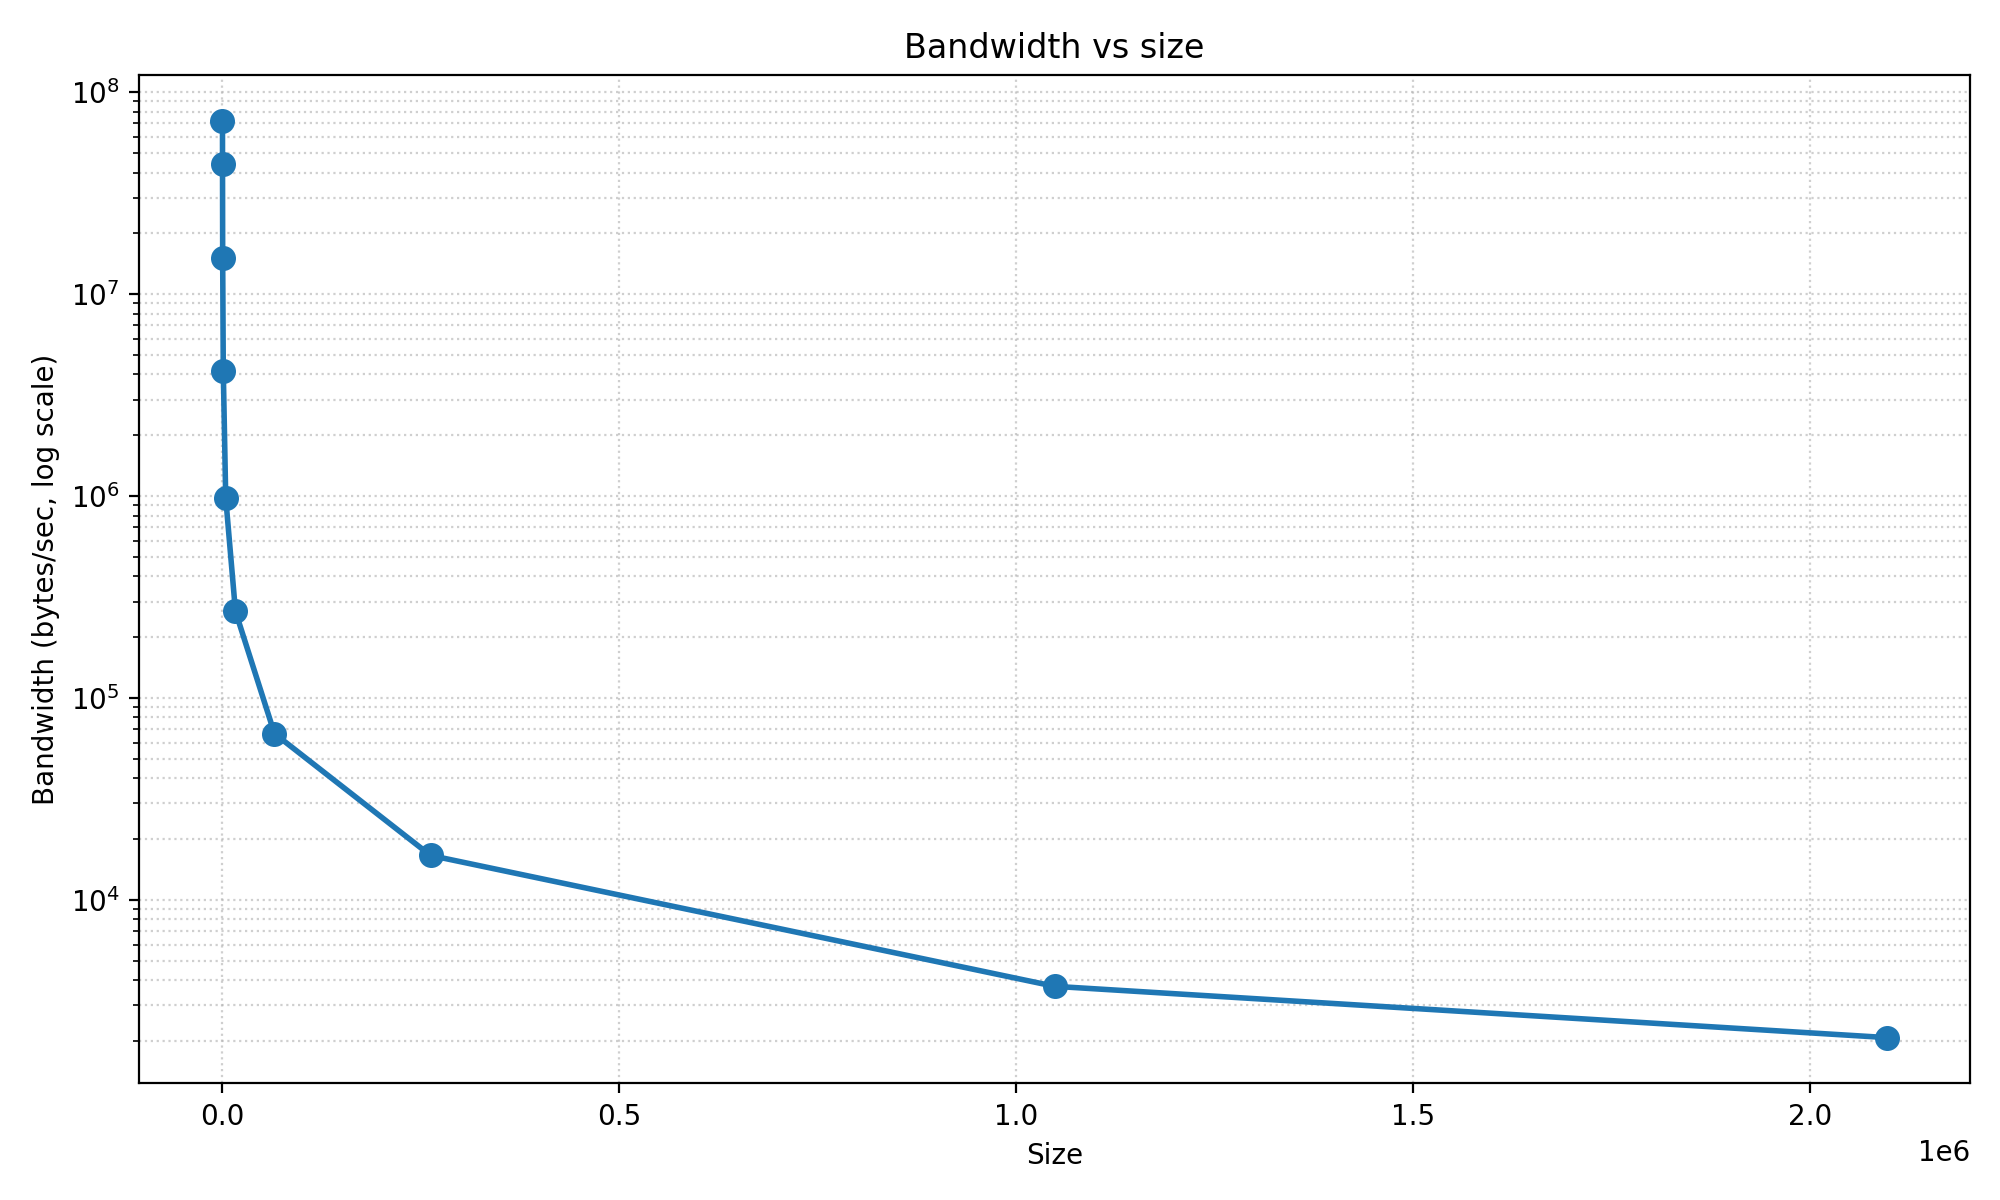
\includegraphics[width=1.0\textwidth]{../noah/plots/6_2/bandwidth_vs_size.png}
    \caption{CPU: Bandwith vs. size of data}
    \label{fig:2}
\end{figure}
\ref{fig:2} shows the bandwith of the kernel of the naive CPU implementation. Measurements are a done with an average over 10 runs.\\
What can be observed is that the bandwith decreases with increasing data sizes. This is due to the fact that, with data getting larger, higher and thus slower levels of the cache hierarchy need to bu used.	
\FloatBarrier
\newpage
\section{GPU reduction: naive}
\begin{figure}[h]
    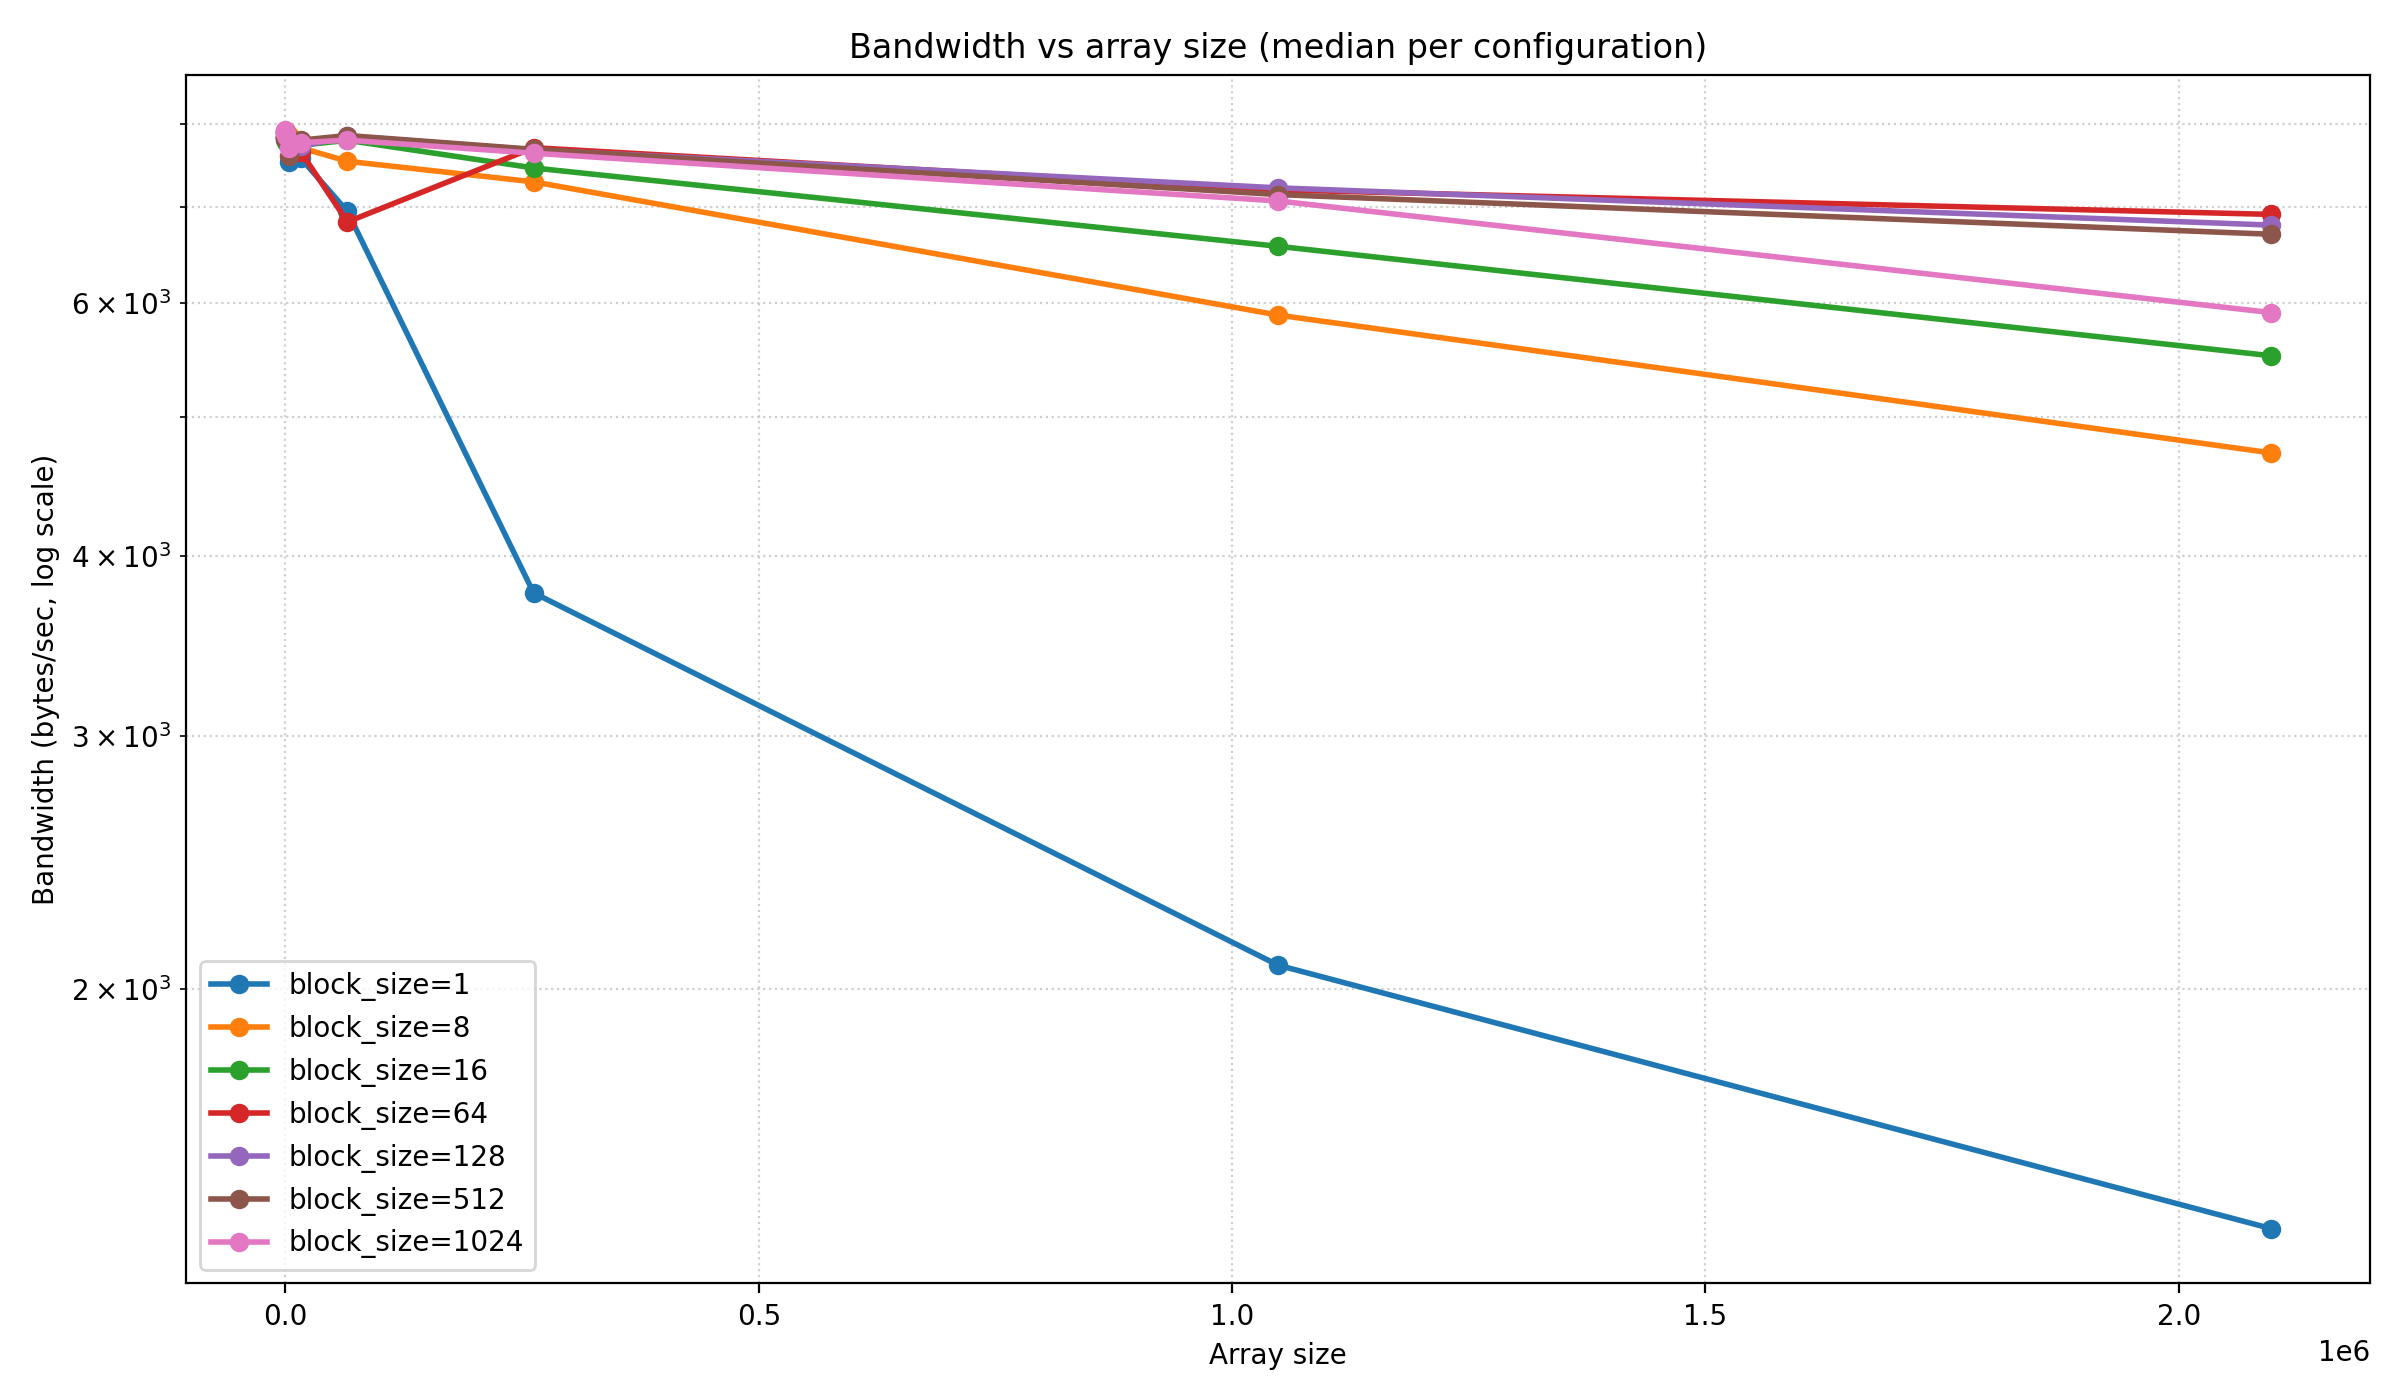
\includegraphics[width=1.0\textwidth]{../noah/plots/6_3/bandwidth_vs_array_size.png}
    \caption{CPU: Bandwith vs. size of data}
    \label{fig:3}
\end{figure}
\ref{fig:3} shows the bandwith of the kernel of the naive GPU implementation. Measurements are a done using a median value, since outliers where observed.\\
For smaller block sizes, perfomance drops significantly for larger matrices, since the CUDA cores are underutilized. For the largest blocksize of 1024, performance is slightly worse than for the 64-512 block sizes, which might be due to a reduced flexibility of scheduling warps and the necessity to synchronize the threads within a block.
\FloatBarrier
\newpage
\section{GPU reduction: parallel}
\FloatBarrier
\newpage
\section{GPU reduction: parallel + volta}
\FloatBarrier
\newpage
\section{GPU reduction: profiling}
\FloatBarrier


\end{document}
